\section{模型的比较}
\label{sec:cdist-comparison}

十二个模型各有来历。面对一个具体问题，选择模型时应当先固定取值类型和要回答的问题，再逐项比较试验机制、支撑、参数的作用以及期望和方差。表~\ref{tab:cdist-discrete}和表~\ref{tab:cdist-continuous}把前两节的结果汇总在一起，下面借助它们讨论三种常见的误用：只凭均值相同就互相替代，忽略方差随均值变化的规律，以及忽略矩的存在条件和尾部形状。

\begin{BookInlineTable}
  \centering
  \caption{离散模型。超几何分布一行中$r=K/N$，方差公式要求$N>1$。}
  \label{tab:cdist-discrete}
  \begin{tabular}{llllc}
    \toprule
    分布 & 机制 & 支撑 & 期望 & 方差\\
    \midrule
    $\operatorname{Bern}(p)$ & 一次成败 & $\{0,1\}$ & $p$ & $p(1-p)$\\
    $\operatorname{Bin}(n,p)$ & $n$次独立成败 & $\{0,\dots,n\}$ & $np$ & $np(1-p)$\\
    $\operatorname{Hyp}(N,K,n)$ & 不放回抽$n$个 & 见式~\eqref{eq:cdist-hypergeometric-pmf} & $nr$ & $nr(1-r)\frac{N-n}{N-1}$\\
    $\operatorname{Geom}(p)$ & 等待首次成功 & $\{1,2,\dots\}$ & $1/p$ & $(1-p)/p^{2}$\\
    $\operatorname{Poisson}(\lambda)$ & 稀有事件计数 & $\{0,1,\dots\}$ & $\lambda$ & $\lambda$\\
    \bottomrule
  \end{tabular}
\end{BookInlineTable}

\begin{BookInlineTable}
  \centering
  \caption{连续模型。最后一列是有限的绝对矩$\mathbb{E}\lvert X\rvert^{r}$所允许的阶数$r>0$。}
  \label{tab:cdist-continuous}
  \begin{tabular}{lllll}
    \toprule
    分布 & 支撑 & 期望 & 方差 & 有限矩\\
    \midrule
    $\operatorname{Unif}(a,b)$ & $(a,b)$ & $(a+b)/2$ & $(b-a)^{2}/12$ & 全部\\
    $\operatorname{Exp}(\lambda)$ & $[0,\infty)$ & $1/\lambda$ & $1/\lambda^{2}$ & 全部\\
    $\mathcal{N}(\mu,\sigma^{2})$ & $\mathbb{R}$ & $\mu$ & $\sigma^{2}$ & 全部\\
    $\operatorname{Gamma}(\alpha,\beta)$ & $(0,\infty)$ & $\alpha/\beta$ & $\alpha/\beta^{2}$ & 全部\\
    $\operatorname{Beta}(a,b)$ & $(0,1)$ & $\frac{a}{a+b}$ & $\frac{ab}{(a+b)^{2}(a+b+1)}$ & 全部\\
    $t_{\nu}(\mu,s^{2})$ & $\mathbb{R}$ & $\mu$（$\nu>1$） & $\frac{s^{2}\nu}{\nu-2}$（$\nu>2$） & $r<\nu$\\
    $\operatorname{Laplace}(\mu,b)$ & $\mathbb{R}$ & $\mu$ & $2b^{2}$ & 全部\\
    \bottomrule
  \end{tabular}
\end{BookInlineTable}

\paragraph{同一个均值}
回到开头的生产线，几种记录的均值都是$2$，方差却各不相同：$\operatorname{Bin}(10,0.2)$为$1.6$，$\operatorname{Hyp}(20,4,10)$为$0.842$，$\operatorname{Poisson}(2)$为$2$。连续模型也一样：均值同为$2$的$\operatorname{Exp}(1/2)$方差为$4$，$\operatorname{Gamma}(2,1)$方差为$2$，$\operatorname{Unif}(0,4)$方差为$4/3$，$\mathcal{N}(2,\sigma^{2})$的方差可以是任何正数。

均值和方差都相同也不够。$\operatorname{Geom}(1/2)$的均值为$2$，方差为$(1-1/2)/(1/2)^{2}=2$，与$\operatorname{Poisson}(2)$完全一样。但前者不取$0$，取$1$的概率是$0.5$；后者取$0$的概率是$0.1353$，取$1$的概率是$0.2707$。一个是等待首次成功的次数，一个是稀有事件的个数，两个数值特征重合只是巧合，第~\ref{chap:random-variable-moments}章说过，有限个矩一般不能确定分布。

\paragraph{方差怎样随均值变化}
在每个单参数的族里，均值一变，方差就按固定的规律跟着变。固定$n=10$，二项分布的方差是$m(1-m/10)$，总小于均值$m$；Poisson分布的方差等于均值；几何分布的方差是$m(m-1)$，均值超过$2$后大于均值。连续情形中，指数分布的方差是$m^{2}$，标准差与均值相等；固定形状$\alpha$的Gamma分布方差为$m^{2}/\alpha$；高斯分布的均值和方差则是两个独立的参数。

图~\ref{fig:cdist-mean-variance}把这些关系画在同一张图上，红点是均值为$2$时各模型的方差。对计数而言，方差小于、等于还是大于均值，可以提示背后是有上限的独立试验、稀有事件，还是等待过程。怎样依据观察到的数据判断这一点，属于统计推断的问题。

\begin{BookInlineFigure}
  \centering
  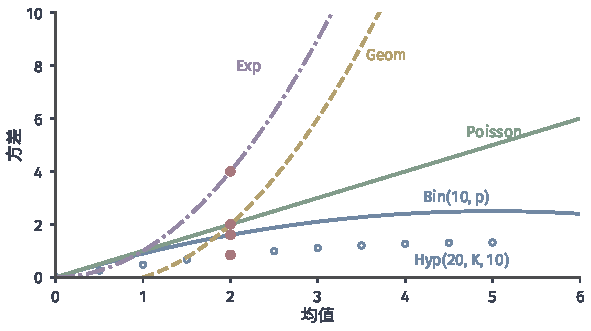
\includegraphics[width=100mm]{figures/07-probability/01-elementary-probability/matplotlib/cdist-mean-variance/figure.pdf}
  \caption{单参数族中方差随均值的变化。$\operatorname{Bin}(10,p)$（蓝线）、$\operatorname{Hyp}(20,K,10)$（蓝色空心点，$K=0,\dots,10$）、$\operatorname{Poisson}$（绿）、$\operatorname{Geom}$（黄，均值不小于$1$）和$\operatorname{Exp}$（紫）。红点是均值为$2$时的方差$0.842$、$1.6$、$2$、$4$，其中$\operatorname{Poisson}(2)$与$\operatorname{Geom}(1/2)$重合于方差$2$。}
  \label{fig:cdist-mean-variance}
\end{BookInlineFigure}

\paragraph{矩的存在与尾部}
表~\ref{tab:cdist-continuous}中只有t分布的矩不全存在。$\nu\leq2$时方差为无穷大，Cauchy分布连期望都没有；这时“均值加减几个标准差”的说法根本无从谈起，只能用中位数和分位数描述位置与离散程度。

即使方差有限，它也不能决定尾部。表~\ref{tab:cdist-tails}把四个方差都为$1$、中心都为$0$的分布放在一起，列出偏离超过$k$个标准差的概率。均匀分布$\operatorname{Unif}(-\sqrt3,\sqrt3)$的支撑有界，超过$\sqrt3$倍标准差的概率就是零；高斯分布的尾部按$\mathrm{e}^{-k^{2}/2}$下降；Laplace分布按$\mathrm{e}^{-\sqrt2k}$下降；$t_3$按幂函数下降。

\begin{BookInlineTable}
  \centering
  \caption{方差为$1$的四种对称分布偏离超过$k$个标准差的概率$\mathbb{P}(\lvert X\rvert>k)$。$t_3$取尺度$1/\sqrt3$。}
  \label{tab:cdist-tails}
  \begin{tabular}{ccccc}
    \toprule
    $k$ & 均匀 & 高斯 & Laplace & $t_3$\\
    \midrule
    $2$ & $0$ & $0.0455$ & $0.0591$ & $0.0405$\\
    $3$ & $0$ & $0.0027$ & $0.0144$ & $0.0138$\\
    $5$ & $0$ & $5.7\times10^{-7}$ & $8.5\times10^{-4}$ & $3.2\times10^{-3}$\\
    \bottomrule
  \end{tabular}
\end{BookInlineTable}

这张表还有一个容易忽略的地方：在$k=2$处，$t_3$的尾概率$0.0405$反而小于高斯的$0.0455$。方差相同时，厚尾分布把更多质量放在中心和极远处，中间一段就要少一些；“尾部更厚”指的是足够远处的行为，并不是在每个阈值上概率都更大。第~\ref{chap:tail-probabilities}章将在只知道均值、方差或更高阶矩时，研究对所有分布都成立的尾概率上界，这些精确值正好用来检验上界的松紧。

\paragraph{边界、特例与极限}
参数取到端点时，模型会退化或变成另一个模型。图~\ref{fig:cdist-family-map}把本章出现过的联系画在一起。实线箭头是本章证明或说明过的构造与极限：$n$个独立Bernoulli变量之和服从二项分布，总体无限增大时超几何趋于二项，$np=\lambda$固定而$n\to\infty$时二项趋于Poisson，步长趋于零时几何等待趋于指数等待，自由度趋于无穷时t密度趋于高斯密度。虚线是族内的特例：$\alpha=1$的Gamma分布是指数分布，$\operatorname{Beta}(1,1)$是均匀分布，$\nu=1$的t分布是Cauchy分布，卡方分布是Gamma分布的子族。

\begin{BookInlineFigure}
  \centering
  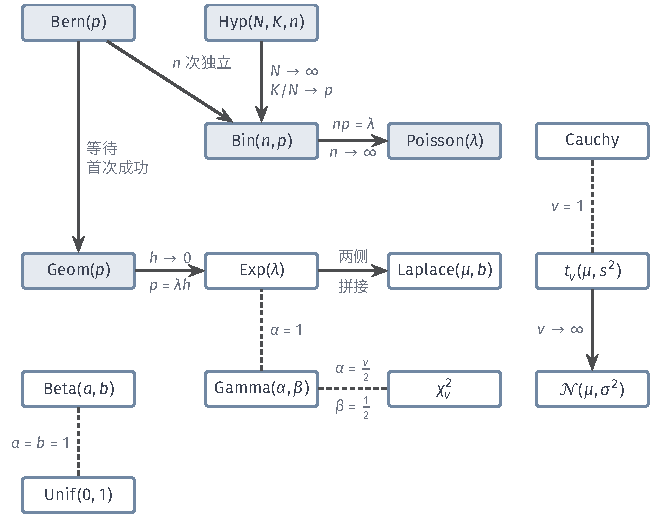
\includegraphics[width=110mm]{figures/07-probability/01-elementary-probability/tikz/cdist-family-map/figure.pdf}
  \caption{本章各一元模型之间的联系。浅蓝框为离散模型，白框为连续模型；实线箭头表示构造或极限，箭头旁注明条件；虚线表示族内的特殊参数值。}
  \label{fig:cdist-family-map}
\end{BookInlineFigure}

每一条极限都附带着近似成立的条件，用近似模型代替原模型时要先核对。二项分布换成Poisson分布，需要机会多而每次稀少，$\operatorname{Bin}(10,0.2)$的零概率就差了近三成；超几何换成二项，需要抽样比例小，否则方差会被高估；t分布换成高斯，在中心附近误差很小，但对任何有限的$\nu$，远处的尾概率都相差数量级。退化的端点（$p=0$或$1$，$n=N$，$K=0$或$N$，$\lambda=0$）则使随机变量成为常数，公式虽然仍可代入，含义要单独理解。

\paragraph{选择的次序}
综合起来，选择一元模型可以按这样的次序检查。先看取值：是计数、等待次数、连续的正值、比例，还是可正可负的误差。再看机制：试验次数是否固定，是否放回，各次是否独立，事件是否稀少。然后看参数的含义：哪个是位置，哪个是尺度，哪个改变形状，率与尺度用的是哪种写法。最后核对需要的矩是否存在、尾部是否合理。只有均值或只有均值和方差相同，不足以让一个模型代替另一个。
